\documentclass[12pt]{article}
\usepackage[a4paper, total={6in, 8.5in}]{geometry}
\usepackage[final]{graphicx}
\usepackage{amsmath}
\usepackage{minted}
\usepackage{multicol}
\usepackage{subcaption}
\usepackage{tabularx}
\usepackage[english]{babel}

\title{Determining the regulation of a transformer when load is resistive.}
\author{}
\date{}

\begin{document}
\vspace*{\fill}
\begin{center}

    \emph{Heaven's Light is Our Guide} \\
    \textbf{Rajshahi Universiy of Engineering and Technology} \\

    \begin{figure}[h]
        \centering
        
\includegraphics[scale=.34]{images/RUET_logo.png}
        \label{fig:ruet_logo}
    \end{figure}
    \vspace{5mm}

    \textbf{Course Code}\\
    ECE 2208\\
    \vspace{3mm}
    \textbf{Course Title}\\
    Electrical Machines - I Sessional

    \vspace{5mm}
    \textbf{Experiment Date:} {October 4, 2023,}\\
    \textbf{Submission Date:} {October 18, 2023}\\

    \vspace{5mm}
    \textbf{Lab Report 1:} Polarity test of a transformer.\\

    \vspace{15mm}

    \begin{tabular}{c|c}
        \textbf{Submitted to} & \textbf{Submitted by} \\
        Md. Omaer Faruq Goni  & Md. Tajim An Noor     \\
        Lecturer              & Roll: 2010025         \\
        Dept of ECE, RUET     &                       \\
    \end{tabular}

\end{center}
\vspace*{\fill}

\pagebreak

\maketitle
\section{Introduction}
\subsection*{Voltage regulation}
Voltage regulation is the measure of how well a transformer can maintain a constant secondary voltage under varying load conditions, as the output secondary voltage may not be what we expect.\\\\
Voltage Regulation of single-phase transformers is the percentage (or per unit value) change in its secondary terminal voltage compared to its original no-load voltage under varying secondary load conditions.\cite{trans}


\subsection*{Circuit Diagrams}
\begin{figure}[htbp!]
    \centering
    % 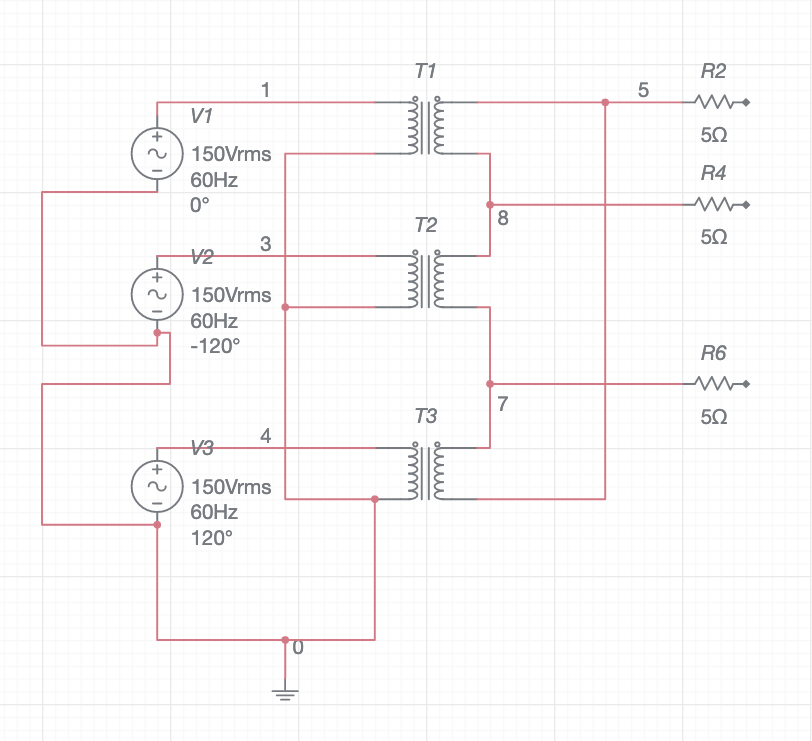
\includegraphics[width=.8\linewidth]{images/output/ydel.png}
    \caption{Circuit diagrams for Y-$\Delta$ three transformer connection.}
    \label{fig:fig}
\end{figure}
\vspace{\fill}

\pagebreak
\section{Tools Used}
\begin{itemize}
    \item Single Phase Transformer (150V - 1A)
    \item Connecting wires
    \item Ammeter (0A - 5A)
    \item Voltmeter (0V - 120V)
    \item Wattmeter
    \item Single Phase AC supply (220V)
    \item Variac (0-250V)
\end{itemize}

\section{Data \& Calculation}
\subsection{Data Table:}
\begin{table}[H]
    \centering
    \caption{No Load}
    \begin{tabular}{|c|c|c|c|c|}
        \hline
        \bf{V\textsubscript{P}} & \bf{V\textsubscript{S}} & \bf{I\textsubscript{P}} & \bf{I\textsubscript{S}} & \bf{W} \\
        \hline
        150.6                   & 139.2                   & 1.34                    & 1.275                   & 182.5  \\
        \hline
    \end{tabular}
\end{table}
\begin{table}[H]
    \centering
    \caption{Full Load}
    \begin{tabular}{|c|c|c|c|c|}
        \hline
        \bf{V\textsubscript{P}} & \bf{V\textsubscript{S}} & \bf{I\textsubscript{P}} & \bf{I\textsubscript{S}} & \bf{W} \\
        \hline
        150.6                   & 131.7                   & 1.42                    & 1.375                   & 195    \\
        \hline
    \end{tabular}
\end{table}

\subsection{Calculation:}
No Load Voltage,\[V_{No-Load} = 139.2V\]\\
Full Load Voltage,\[V_{Full-Load} = 131.7V\]\\
Voltage Regulation,
\begin{align*}
    \%V\!R & = |\frac{\text{V\textsubscript{No-Load}}-\text{V\textsubscript{Full-Load}}}{\text{V\textsubscript{No-Load}}}|\times 100\% \\
           & = |\frac{139.2-131.7}{131.7}|\times 100\%                                                                                 \\
           & = 5.69\%
\end{align*}
\subsection{Result}

Voltage Regulation, \(\%V\!R = 5.69\%\)

\section{Discussion}
Voltage regulation controls how much the secondary terminal voltage inside the transformer varies due to changes in the connected load. If these losses are significant and the secondary voltage drops too low, the transformer's efficiency and performance are impacted.\\
When no load is attached to the transformer's secondary winding, there is no closed-loop situation, hence there is no output load current and the transformer behaves as a single winding with a high self-inductance.\\
Loading the secondary winding with a simple load causes a secondary current to flow, at any power factor(depending on the type of load, here resistive), through the internal winding of the transformer. Thus voltage drops due to the windings internal resistance and its leakage reactance causes the output terminal voltage to change.\\
So, whenever load is attached, full potential of the transformer can't be achieved, there will be some loss. Voltage regulation helps to determine that.

\section{Conclusion}
Since this experiment was done with AC supply, utmost caution was exercised to avoid any accident. To avoid electrocution, help from lab assistants was taken.
\bibliographystyle{IEEEtran}
\bibliography{ref}

\end{document}